\chapter{Introduzione alla biometria}

\section{Riconoscimento biometrico e tecniche tradizionali}

\subsubsection{Nuovo modo di identificare e autenticare}

La biometria ci offre un nuovo modo, \textbf{automatico}, di identificare le persone.

Si passa da una cosa che \textbf{sappiamo} (password) o che \textbf{abbiamo} (documento, chiave), a ciò che \textbf{siamo} (iride, impronta) o ciò che \textbf{facciamo} (voce, firma).

\subsubsection{Definizione di biometria}

Si definisce biometria un \textbf{insieme di tecniche automatiche per il riconoscimento degli individui} basato sulle loro caratteristiche \textbf{fisiche} e \textbf{comportamentali}.

\subsection{Riconoscimento}

Il riconoscimento della identità è l'operazione che assoccia una identità a un individuo.

Il riconoscimento può essere diviso in due categorie:
\begin{itemize}
    \item Verifica dell'identità (\textbf{autenticazione})
    \item Ricerca dell'identità (\textbf{identificazione})
\end{itemize}
Queste due categorie hanno diversa funzione e complessità.

\subsubsection{Autenticazione}

La verifica dell'identità equivale a rispondere alla domanda: \textbf{sono chi dico di essere?}

Si può dunque confermare o negare l'identità dichiarata dall'utente; viene fatto con metodi one-to-one (1:1).

\subsubsection{Identificazione}

La ricerca dell'identità equivale a rispondere alla domanda: \textbf{Chi sono io?}

Si deve dunque stabilire l'identità del soggetto
\begin{itemize}
    \item da un insieme di identità note (problema di identificazione \textbf{chiuso})
    \item in altre situazioni (problema di identificazione \textbf{aperto})
\end{itemize}
La ricerca dell'identità avviene con metodi one-to-many (1:N).

\subsubsection{Autenticazione/Identificazione Positiva e Negativa}

\begin{itemize}
    \item \textbf{Positiva:} consiste in quando si cerca di stabilire con elevata accuratezza che l'utente sia chi dice di essere.
    \item \textbf{Negativa:} consiste in quando si cerca di stabilire con elevata accuratezza che l'utente non sia chi dice di essere.
\end{itemize}

Alcuni esempi:
\begin{itemize}
    \item Un sistema di accesso ad un sito militare controlla la mia iride
    per controllare se appartengo ad un lista di abilitati all’ingresso. \textbf{(Identificazione positiva)}
    \item Un sistema di visione controlla con delle telecamere se chi
    passa davanti agli obiettivi non sia un terrorista presente in
    una lista. \textbf{(Identificazione negativa)}
    \item Al bancomat si controlla se chi sta usando la carta sia
    effettivamente il possessore della carta. \textbf{(Autenticazione positiva)}
\end{itemize}

\subsection{Metodi classici di autenticazione}
I metodi classici di autenticazione si basano su due principali attività:
\begin{itemize}
    \item \textbf{Possesso:} basate su qualcosa che possiedi (token-based); posso entrare in laboratorio se possiedo la chiave
    \item \textbf{Conoscenza} di una porzione informazione: qualcosa che sai; posso accedere alla rete se conosco la password
\end{itemize}
Alcuni sistemi utilizzano in modo \textbf{ibrido} queste due modalità; usi il bancomat se \textbf{hai} la carta e \textbf{conosci} il PIN.

\subsubsection{Metodi classici: problemi}

\begin{itemize}
    \item  \textbf{Metodi basati sul possesso}
    
    Il token può essere:
    \begin{itemize}
        \item perso o rubato
        \item prestato a chi non dovrebbe usarlo
        \item usato in contesti non autorizzati
    \end{itemize}
    \item \textbf{Metodi basati sulla conoscenza}
    
    La password può essere:
    \begin{itemize}
        \item dimenticata
        \item ceduta o trasmessa ad altri
        \item individuata per tentativi
    \end{itemize}
\end{itemize}

È stato provato che mediamente una persona deve ricordare oltre 20 password/codici; ne consegue che si tende ad usare la stessa password ovunque.

\subsection{Metodi biometrici}

Con i metodi biometrici il riconoscimento avviene in base alle caratteristiche fisiche e/o comportamentali dell’individuo:
\begin{itemize}
    \item \textbf{Tratti fisici}

    \begin{itemize}
        \item iride
        \item impronta
        \item geometria della mano
        \item volto
    \end{itemize}
    \item \textbf{Tratti comportamentali}

    \begin{itemize}
        \item voce
        \item firma
        \item camminata
    \end{itemize}
\end{itemize}

In figura \ref{fig:trad-vs-bio} viene confrontato il livello di sicurezza delle modalità che sono state trattate.

\begin{figure}
    \centering
    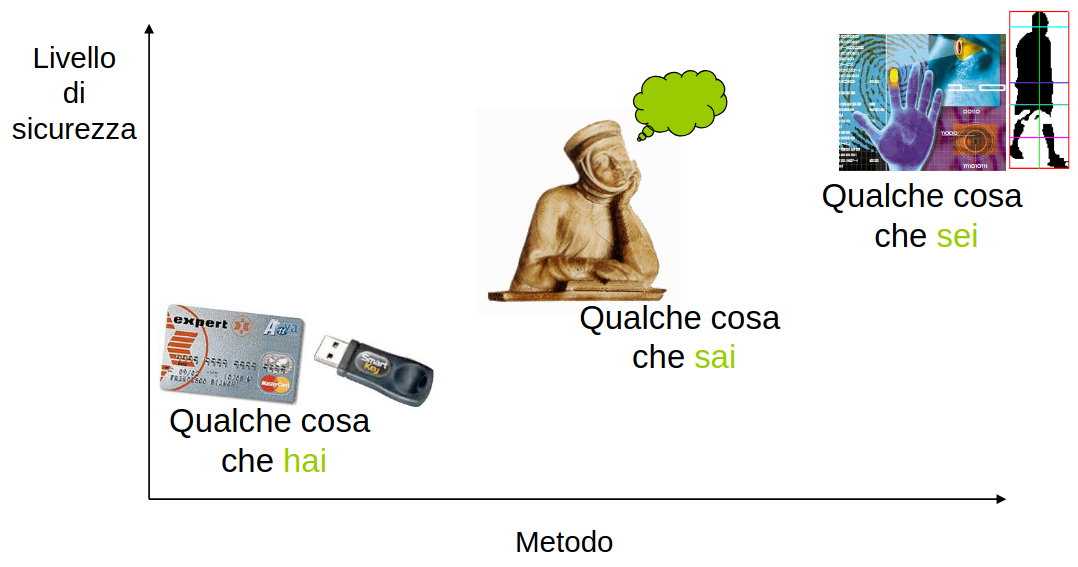
\includegraphics[width=0.75\linewidth]{chapters/images-chap1/tradizionali_vs_biometrici.png}
    \caption{Confronto del livello di sicurezza delle modalità viste}
    \label{fig:trad-vs-bio}
\end{figure}

\subsubsection{Alcuni vantaggi}

\begin{itemize}
    \item i tratti sono sempre con te, \textbf{non possono essere dimenticati} o usati da altri.
    \item è molto più \textbf{difficile falsificare} un tratto biometrico che un documento o una chiave
    \item l'\textbf{accuratezza} della identificazione può essere molto più \textbf{elevata} dei metodi tradizionali
    \item possono essere \textbf{combinati} con i metodi tradizionali
    \item solo i metodi biometrici possono realizzare una \textbf{identificazione negativa} (\textit{"il sistema dice che io non sono lui"})
    \item riducono (quasi a zero) la possibilità di reclami di \textbf{ripudazione} (\textit{"sono innocente..qualche altra persona ha usato il mio PIN.."})
\end{itemize}

\subsubsection{Alcuni svantaggi}

\begin{itemize}
    \item i sistemi biometrici hanno un \textbf{costo maggiore}
    \item i sistemi biometrici rispondono in realtà con un \textbf{livello di matching} e rispondo con una decisione binaria yes/no
    \item alcune persone li vedono come una \textbf{invasione della privacy}
    \item non possono essere cambiati a piacimento
    \item alcune persone non possiedono tutti i tratti biometrici (mancanza di iride, impronte usurate, senza voce...)
\end{itemize}

\subsubsection{Biometrics and Biometry}

In inglese esistono due termini che in italiano corrispondono al termine biometria:
\begin{itemize}
    \item \textbf{Biometrics:} metodi di identificazione automatica basati sulle caratteristiche fisiche e comportamentali dell'individuo.
    \item \textbf{Biometry:} campo di studio molto più ampio che comprende l'applicazione della statistica alla biologia e alla medicina.
\end{itemize}

\subsubsection{Le 7 proprietà del tratto biometrico}

\begin{itemize}
    \item \textbf{Universalità:} ogni persona deve possedere questo tratto o caratteristica
    \item \textbf{Unicità:} due persone non devono avere lo stesso tratto uguale
    \item \textbf{Permanenza:} la caratteristica deve essere invariante nel tempo
    \item \textbf{Misurabilità:} il tratto deve poter essere esaminato quantitativamente
    \item \textbf{Performabilità:} accuratezza della identificazione che deve essere adeguata e deve essere garantita senza particolari condizioni operative
    \item \textbf{Accettabilità:} percentuale di persone che potrebbero accettare l'uso del sistema biometrico
    \item \textbf{Circonvezione:} grado di difficoltà nell'ingannare il sistema con tecniche fraudolente
\end{itemize}

\section{Aspetto e funzionamento dei sistemi biometrici}

\subsubsection{Enrollment}

È la \textbf{fase di inserimento}, il tratto biometrico viene per la prima volta acquisito dal sistema e registrato oppure viene creato il documento biometrico.

\subsubsection{Identificazione/Verifica}

È la \textbf{fase di riconoscimento}, il tratto biometrico viene nuovamente acquisito. Se risulta sufficientemente aderente alle informazioni registrate nel sistema biometrico l'accesso viene consentito.

In figura \ref{fig:enroll-ident} vengono mostrate le fasi di enrollment e identificazione.

In figura \ref{fig:matching-score} viene mostrato il concetto di matching score e di soglia.

\begin{figure}
    \centering
    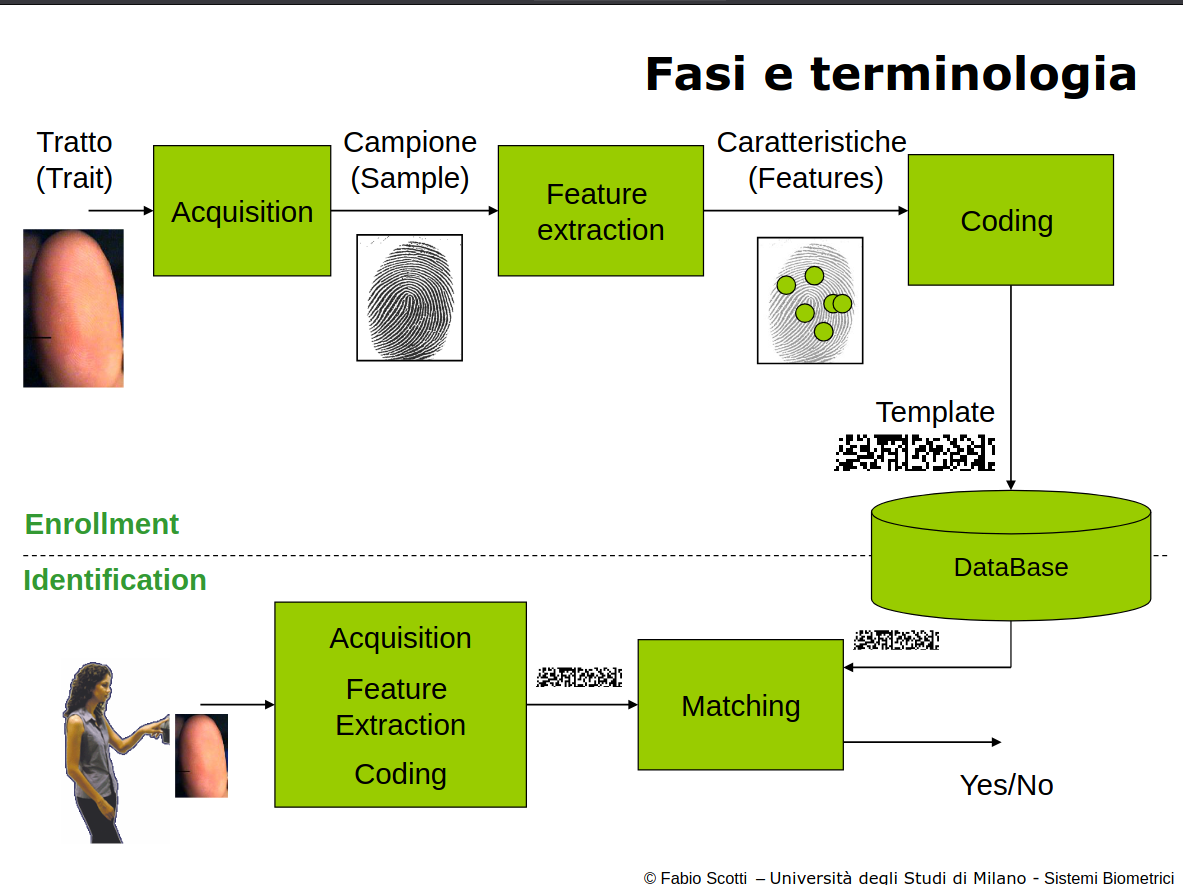
\includegraphics[width=0.95\linewidth]{chapters/images-chap1/enrollment-identification.png}
    \caption{Fasi di Enrollment e Identificazione}
    \label{fig:enroll-ident}
\end{figure}

\begin{figure}
    \centering
    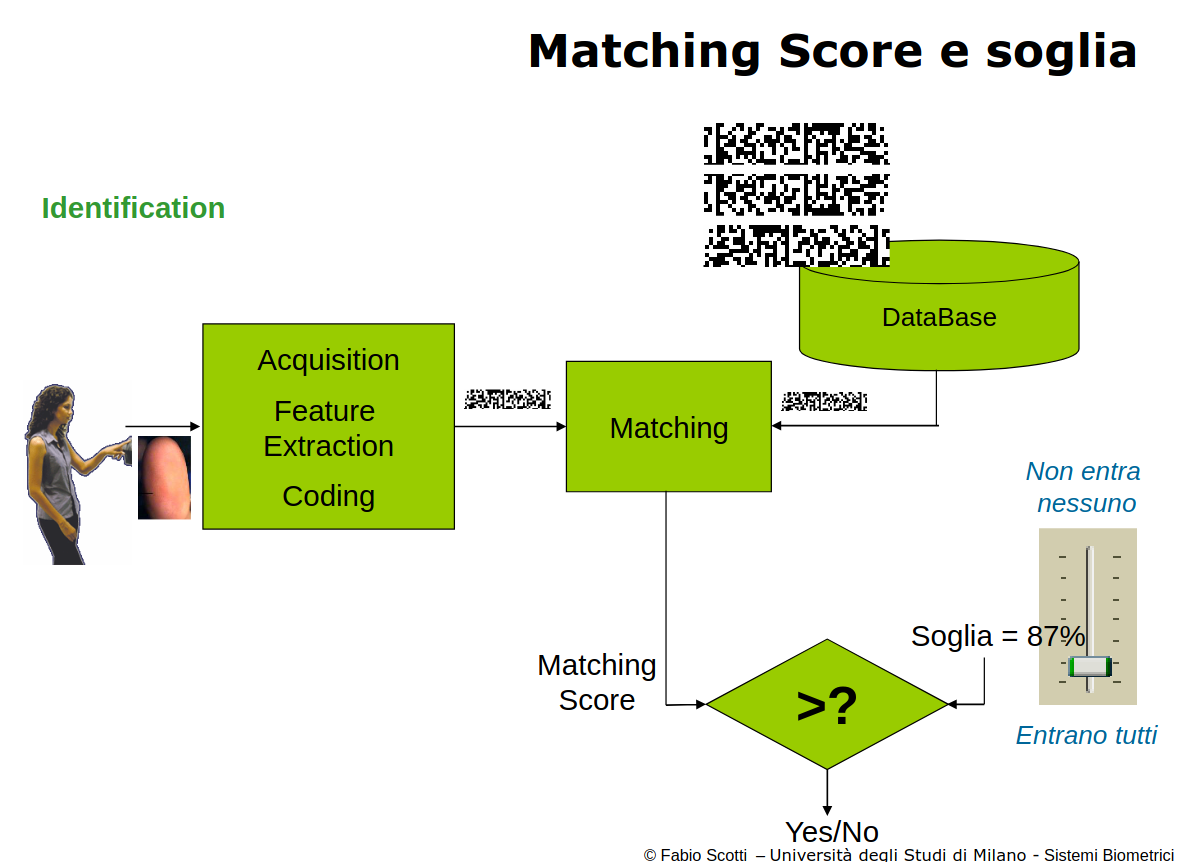
\includegraphics[width=0.95\linewidth]{chapters/images-chap1/matching-score.png}
    \caption{Matching score e soglia}
    \label{fig:matching-score}
\end{figure}

\newpage

\section{Tratti biometrici: caratteristiche}

Tra i tratti biometrici più diffusi e maggiormente impiegati nei sistemi biometrici rientrano:
\begin{itemize}
    \item Impronte
    \item Volto
    \item Iride
    \item Geometria della mano/vene
    \item Voce
    \item Firma
    \item Sistemi multimodali
\end{itemize}
Iniziamo ad approfondire quelli maggiormenti utilizzati.

\subsubsection{Impronta digitale}
È il tratto biometrico più antico e diffuso del mondo. Si tratta di un pattern di creste e valli che si sviluppa da una configurazione casuale già presente dall'embrione. Ad oggi, si ritiene che siano uniche e che il pattern non cambi nel tempo.

Per rilevarle vengono usati sensori:
\begin{itemize}
    \item Termici
    \item Ultrasuoni
    \item Capacitivi
    \item Ottici
    \item Scanner tradizionali
\end{itemize}

Il riconoscimento avviene attravero tre approcci, mostrati in figura \ref{fig:trad-vs-bio}.

\begin{figure}
    \centering
    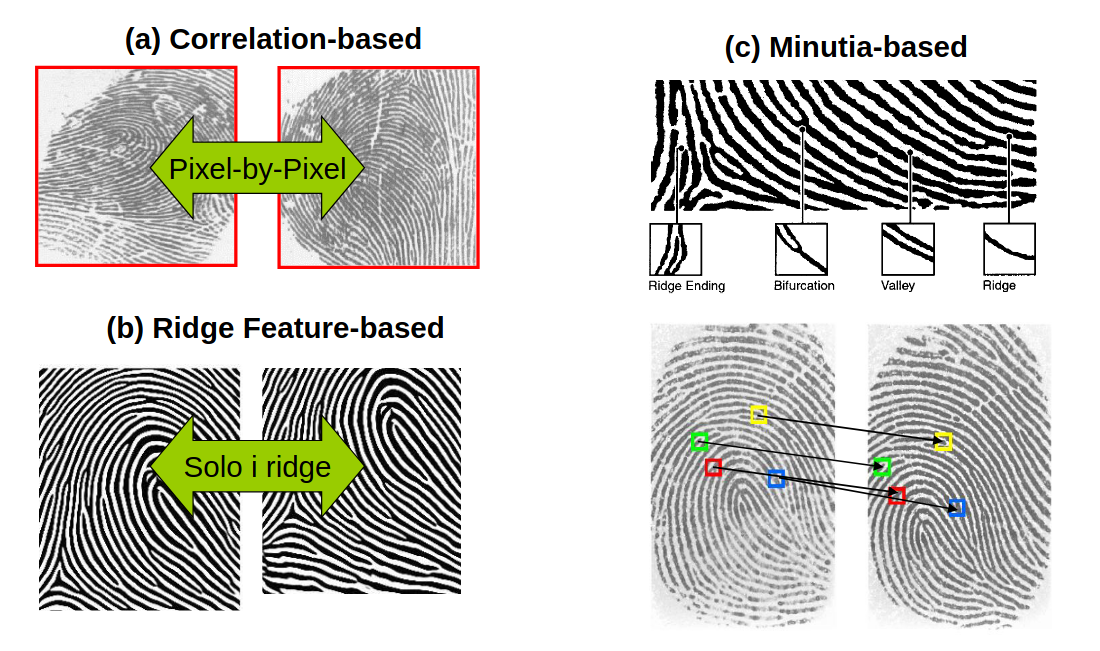
\includegraphics[width=1\linewidth]{chapters/images-chap1/impronte.png}
    \caption{Approcci di riconoscimento delle impronte}
    \label{fig:impronte}
\end{figure}

\subsubsection{Volto}

È uno tra i tratti biometrici meno invasivi; viene usato per riconoscere le persone in una grandissima varietà di applicazioni.

I sensori utilizzati per rilevare questo tratto sono:
\begin{itemize}
    \item Telecamere
    \item Macchine fotografiche digitali
    \item Webcam
    \item Smartphone
    \item Scanner 3D
\end{itemize}

È difficile creare dei sistemi che sappiano affrontare efficacemente l'invecchiamento, espressioni del volto, variazioni della posa...

Il riconoscimento avviene con due approcci differenti, mostrati in figura \ref{fig:volto}:
\begin{itemize}
    \item Trasformazione: si crea una "base di immagini" che permette di ricostruire un nuovo viso come una somma di immagini contenute nella base
    \item Attributi: si localizza il volto nell'immagine e si misurano delle caratteristiche (distanza degli occhi, lunghezza del naso, della bocca...)
\end{itemize}

\begin{figure}
    \centering
    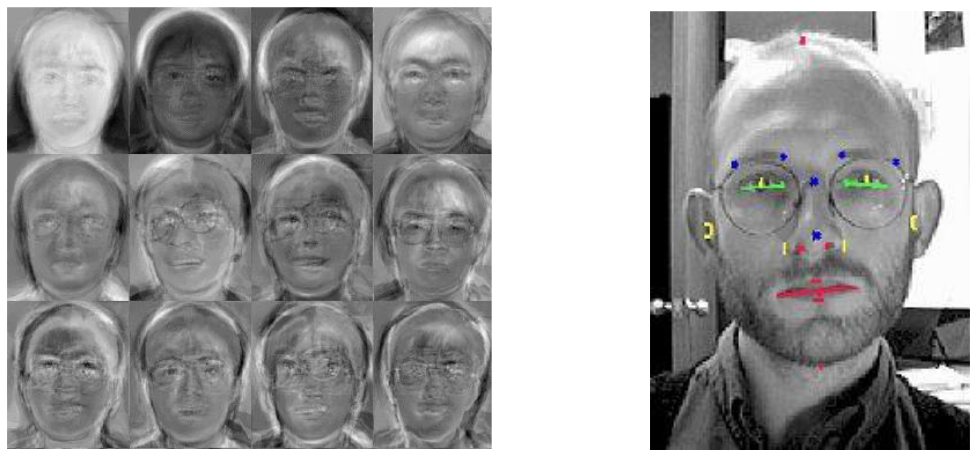
\includegraphics[width=1\linewidth]{chapters/images-chap1/volto.png}
    \caption{Approcci per il riconoscimento del volto}
    \label{fig:volto}
\end{figure}

\subsubsection{Mano}

È un tratto biometrico ben accettato dagli utenti in quanto è poco invasivo; offre un discreto livello di sicurezza, ed offre la possibilità di controllare più aspetti.

Di solito si lavora su tre viste: palmare, laterale e dorsale.

Per il rilevamento del tratto, si utilizzano degli scanner o delle camere.

Ci sono diversi approcci per il riconoscimento, mostrati in figura \ref{fig:mano}.

\begin{figure}
    \centering
    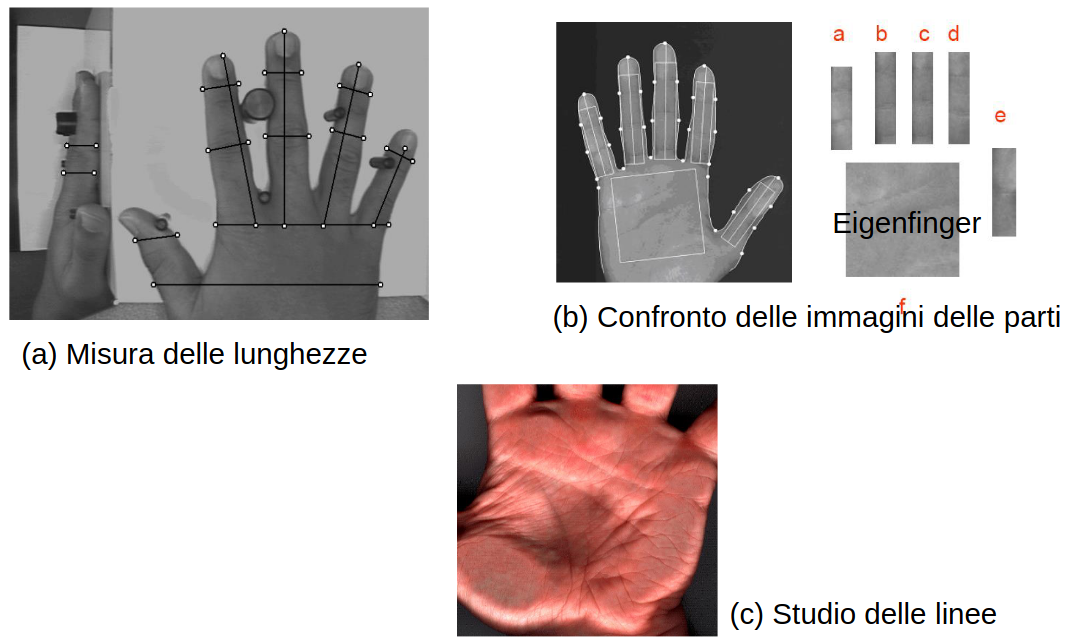
\includegraphics[width=1\linewidth]{chapters/images-chap1/mano.png}
    \caption{Approcci per il riconoscimento della mano}
    \label{fig:mano}
\end{figure}

\newpage

\subsubsection{Iride}

È considerato essere il tratto biometrico più accurato: l'iride presenta numerosissime caratteristiche che sono stabili nel tempo. Si tratta di un sistema piuttosto complesso e costoso, ma difficile da frodare.

Per il rilevamento, vengono utilizzate delle camere ad alta definizione o delle ottiche speciali.

Il sistema possiede degli algoritmi per:
\begin{itemize}
    \item Trovare l'occhio e selezionare la parte utile
    \item Eliminare i riflessi e le ciglia
    \item Compensare le deformazioni dell'iride che si comporta elasticamente con le variazioni di luce
    \item Linearizzazione dell'iride e creazione dell'IRIS CODE
\end{itemize}

\subsubsection{Firma}

È un metodo molto semplice e diffuso; ha una bassa accuratezza e un moderato costo del sensore.

Il riconoscimento è basato sugli andamenti nel tempo di:
\begin{itemize}
    \item coordinate (x, y)
    \item pressione
    \item inclinazione
\end{itemize}

\subsubsection{Voce}

È un tratto biometrico accettato dagli utenti; ha una bassa accuratezza e un costo moderato.

\subsubsection{Sistemi multimodali}

Consistono nell'unire più tecnologe biometriche in un sistema per aumentarne l'accuratezza o la robustezza alle frodi.

\newpage

\section{Comparazione dei sistemi biometrici}

Comparare dei sistemi biometrici è un compito complesso, perché vi sono molti parametri di giudizio difficilmente stimabili

\begin{figure}[h]
    \centering
    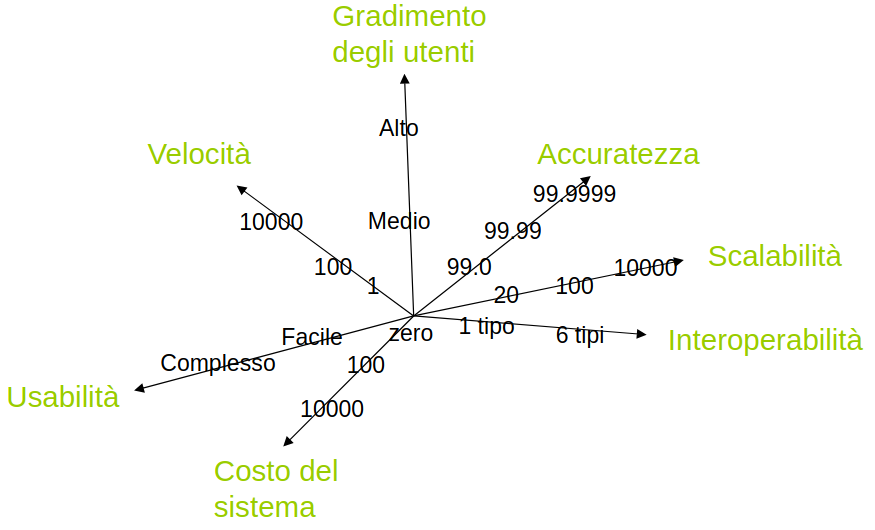
\includegraphics[width=0.95\linewidth]{chapters/images-chap1/comparazione.png}
    \caption{Comparazione tra sistemi biometrici}
    \label{fig:comparazione}
\end{figure}

\subsubsection{Autenticazione/Identificazione}

Ad oggi, solo iride e impronta sono usati per \textbf{identificazione} (1:N) con N grandi. I requisiti per il funzionamento 1:N sono:
\begin{itemize}
    \item accuratezze elevatissime
    \item template in byte ridotti (minore di kB)
    \item tempo per un singolo confronto molto basso (minore di ms)
\end{itemize}

Per questo motivo mano, voce, volto e firma vengono usati solo per \textbf{autenticazione} (1:1) o identificazione (1:N) con N solo qualche decina di persone.

\subsubsection{Variazioni del tratto}

Occore tenere presente se un un tratto biometrico cambia nell'arco di una vita o giorno dopo giorno; i tratti biometrici già formati dalla nascita e stabili per tutta la vita sono iride e impronta.

L'alta variabilità del tratto biometrico nel tempo produce una peggiore accuratezza del sistema biometrico.

\subsubsection{Velocità del sistema}

Si calcola il \textbf{tempo misurato in secondi per eseguire completamente un singolo matching}, da cui si può stimare il \textbf{numero di utenti massimo identificabile/autenticabili in un'ora.}

Ad esempio:
\begin{itemize}
    \item abbiamo 2000 iridi registrate in un sistema come persone indesiderate (N=2000)
    \item Vogliamo che la persona venga identificata negativamente in 2 secondi
\end{itemize}
Ne consegue che il tempo per eseguire un singolo matching deve essere minore di 1ms.

I sistemi possono funzionare:
\begin{itemize}
    \item \textbf{in tempo reale:} la velocità è cruciale (ad esempio aereoporto)
    \item \textbf{offline:} la velocità è importante ma non cruciale (ricerca di impronte in un archivio)
\end{itemize}

\subsubsection{Interoperabilità}

È la capacità di un sistema biometrico di funzionare anche con sample biometrici acquisiti con sensori di diverso tipo usando lo stesso tratto biometrico.

L'interoperabilità diventerà sempre più importante dato che il \textbf{tipo} di sensori è \textbf{destinato ad aumentare nel tempo}.

\begin{figure}[h]
    \centering
    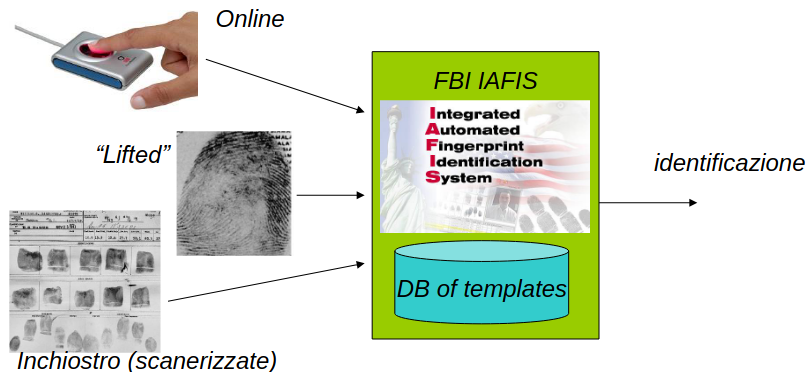
\includegraphics[width=0.95\linewidth]{chapters/images-chap1/interoperabilita.png}
    \caption{Un esempio di interoperabilità}
    \label{fig:interoperabilita}
\end{figure}

\newpage

\section{Impiego di un sistema biometrico: aspetti di privacy e legislativi}

\subsubsection{Percezione degli utenti}

L'uso delle tecnologie biometriche viene spesso percepito dagli utenti in modo duplice:
\begin{itemize}
    \item \textbf{Vantaggi:}
    \begin{itemize}
        \item non devo avere chiavi o ricordare codici (1)
        \item sarà più difficile rubarmi i soldi dal bancomat (2)
        \item funzionerà contro il terrorismo (3)
    \end{itemize}
    \item \textbf{Svantaggi:}
    \begin{itemize}
        \item le mie impronte saranno schedate (1)
        \item sapranno dove vado (2)
        \item sapranno che cosa compro (3)
    \end{itemize}
\end{itemize}

\subsubsection{Discussione sui vantaggi}
\begin{itemize}
    \item \textbf{(1): VERO}
    \item \textbf{(2): PARZIALMENTE VERO;} esistono modi per frodare un sistema biometrico, ma sono molto complessi. La tecnologia anti-spoofing procede di pari passo con quella di spoofing
    \item \textbf{(3): PARZIALMENTE VERO;} il problema delle identità multiple e dei documenti falsi vieno quasi azzerato, ma rimane il problema della fonte (anello debole)
\end{itemize}

\subsubsection{Discussione sugli svantaggi}
\begin{itemize}
    \item \textbf{(1): PARZIALMENTE VERO;} le tecnologie sono simili, cambiano i DB ed il loro impiego
    \item \textbf{(2): GIÀ VERO OGGI;} ad esempio Telepass, pagamenti online di biglietti o prenotazioni
    \item \textbf{(3): GIÀ VERO OGGI;} bancomat/carte di credito
\end{itemize}

\subsubsection{L'anello debole della catena}

L'anello debole della catena di identificazione rimane anche se usiamo le tecnologie biometriche: \textbf{il problema è la fonte}.

Un documento biometrico nasce da altri documenti tradizionali: ad esempio, per il passaporto biometrico serve un documento di riconoscimento valido.

\subsubsection{Sample o Template?}

\textbf{Sample:}
\begin{itemize}
    \item \textbf{PRO:}
    \begin{itemize}
        \item può essere nuovamente filtrato, analizzato
        \item permette cambi tecnologici
    \end{itemize}
    \item \textbf{CONS:}
    \begin{itemize}
        \item occupa più spazio
        \item dato utile per attacchi con fake
        \item lede la privacy
    \end{itemize}
\end{itemize}

\begin{figure}[h]
    \centering
    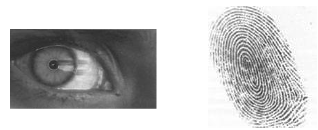
\includegraphics[width=0.5\linewidth]{chapters/images-chap1/sample.png}
    \caption{Sample}
    \label{fig:sample}
\end{figure}

\textbf{Template:}
\begin{itemize}
    \item \textbf{PRO:}
    \begin{itemize}
        \item minore elaborazione durante la verifica
        \item minore occupazione in memoria e banda in trasmissione
        \item protegge meglio la privacy
    \end{itemize}
    \item \textbf{CONS:}
    \begin{itemize}
        \item legato alla tecnologia che lo ha generato
        \item difficilmente migliorabile
    \end{itemize}
\end{itemize}

\begin{figure}
    \centering
    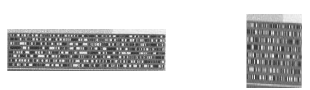
\includegraphics[width=0.5\linewidth]{chapters/images-chap1/template.png}
    \caption{Template}
    \label{fig:template}
\end{figure}

\subsubsection{Il problema della proscrizione}

Quando un dato biometrico è inviato ad un dato sistema, l'informazione contenuta \textbf{non dovrebbe essere utilizzata per altri scopi} se non dell'uso richiesto dall'utente.
Ad esempio, si può essere controllati se si appartiene ad una particolare lista.

Il problema delle liste di proscrizione \textbf{non} è presente solo nei sistemi biometrici; tuttavia le tecniche biometriche possono peggiorare la situazione perché il matching biometrico è molto \textbf{difficile da ripudiare}.

\textbf{La biometria prolunga la l'intervallo di tempo nel quale fare il riconoscimento}.

\subsubsection{Privacy e variazioni del tratto}

Usare un tratto biometrico che varia molto nel tempo tende a produrre falsi negativi (il sistema dice che non sono io).

Allora perché non usare sempre iride ed impronta dato che hanno i tassi di errore fra i più bassi?
\begin{itemize}
    \item costo del sistema
    \item è corretto adattare l'invasività del tratto e l'accettazione degli utenti con il grado di sicurezza richiesto
    \item usare un tratto che varia nel tempo può proteggere dall'effetto "schedatura"
\end{itemize}

\subsection{Decalogo del garante sulla biometria}

\textbf{"Il decalogo è una guida operativa per chi progetta e costruisce sistemi per la rivelazione di dati corporei} e per ogni cittadino che deve segnalare ogni abuso".
\begin{enumerate}
    \item \textbf{Affidabilità del sistema} di rivelazione dei dati corporei, indicando il suo livello di accuratezza
    \item \textbf{Informativa chiara}, lasciando la libertà di aderire o meno al sistema (salvo stringenti ragioni)
    \item \textbf{Liceità} verificabile sotto i profili di necessità, finalità, correttezza.
    \item \textbf{Deroga motivata} con uso controllato in speciali casistiche
    \item \textbf{Delimitata memorizzazione} su supporti sempre disponibili per l'interessato e non centrilizzazione
    \item \textbf{Temporanea conservazione} in ordine cronologico per il necessario tempo limitato
    \item \textbf{Scrupolose misure di sicurezza} con sistemi inequivoci e senza rischio (con un vigilatore dei dati indipendente)
    \item \textbf{Piena ed immediata conoscibilità dei dati biometrici da parte dell'interessato}
    \item \textbf{Rispetto rigoroso} delle norme aggiornate al \textbf{GDPR europeo 2018}
    \item \textbf{Disattivazione automtica, immediata e certa di funzioni di smart card o analoghe} nel caso di smarrimento o furto
\end{enumerate}

\subsection{GDPR}

\textbf{General Data Protection Regulation.}

Definisce i dati biometrici come una categoria speciale di dati personali e proibisce la loro elaborazione e memorizzazione presso terze parti senza il consenso

\subsubsection{Pesudonomizzazione}

\textit{Il trattmento dei dati personali in modo tale che:}
\begin{enumerate}
    \item \textit{i dati non possano essere più attribuiti ad un interessato specifico senza l'utilizzo di informazioni aggiuntive} \textbf{(assenza di identificabilità diretta del soggetto interessato)}
    \item \textit{a condizione che tali informazioni aggiuntive siano conservate separatamente} \textbf{(l'adozione di misure di sicurezza ulteriori da aggiungenre alla pseudonimizzazione, come ad esempio la cifratura)}
    \item \textit{e soggette a misure tecniche e organizzative intese a garantire che tali dati personali non siano attirbuiti a una persona fisica indetificata o identificabile} 
\end{enumerate}

Viene garantita la \textbf{ricostruibilità} dei processi di mascheramento dell'identità, permettendo la reidentificazione e assicurando dunque \textbf{l'accountability} (processo con cui si è chiamati a rendere conto delle conseguenze delle proprie azioni).

\subsubsection{Resilienza}

È la \textbf{capacità di un sistema di adattarsi alle condizioni d'uso in modo da garantire la disponibilità dei servizi erogati per un lasso di tempo adeguato.}

